\section{Sri Rahayu(1174015)}
\subsection{Instalasi Map Server}
\begin{enumerate}
    \item Download terlebih dahulu map servernya. Untuk webnya bisa \href{https://mapserver.org/}{Klik disini} atau \href{https://ms4w.com/}{Klik disini} Untuk windows.
    \hfill\break
    \begin{figure}[H]
		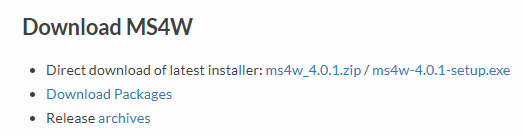
\includegraphics[width=4cm]{figures/1174015/4/No1.png}
		\centering
		\caption{Download File MS4W}
    \end{figure}
    \hfill\break

    \item Setelah di download, bisa langsung melakukan Instalasi. Untuk versi windows bisa saya sarankan mendownload yang .exe agar lebih mudah saat instalasi.
    \hfill\break
    \begin{figure}[H]
		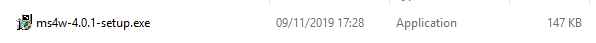
\includegraphics[width=4cm]{figures/1174015/4/No2.png}
		\centering
		\caption{Install File exe}
    \end{figure}
    \hfill\break

\end{enumerate}


\subsection{Konfigurasi Map Server}
Jika telah selesai melakukan instalasi kita akan melakukan konfigurasi
\begin{enumerate}
  \item Buka folder ms4w. Masuk ke folder apache
  \hfill\break
    \begin{figure}[H]
		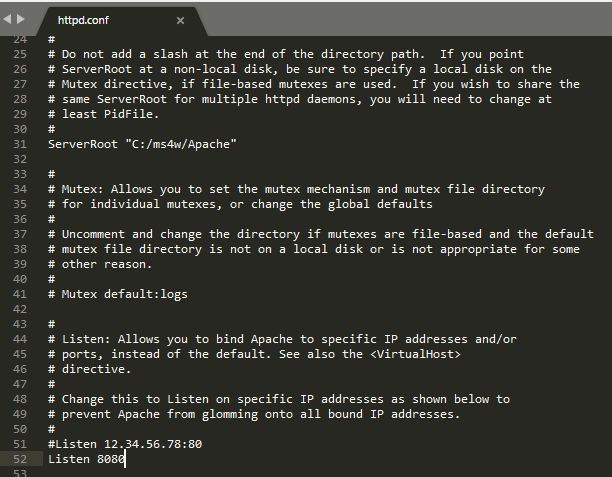
\includegraphics[width=4cm]{figures/1174015/4/No3.png}
		\centering
		\caption{Isi Folder apache}
    \end{figure}


  \item Masuk ke folder conf
  \hfill\break
    \begin{figure}[H]
		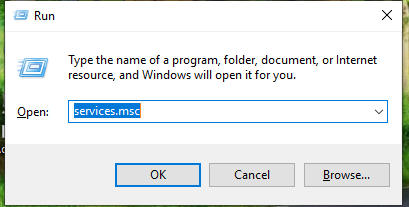
\includegraphics[width=4cm]{figures/1174015/4/No4.png}
		\centering
		\caption{Folder conf}
    \end{figure}
  \item Masuk ke folder conf
  \hfill\break
    \begin{figure}[H]
		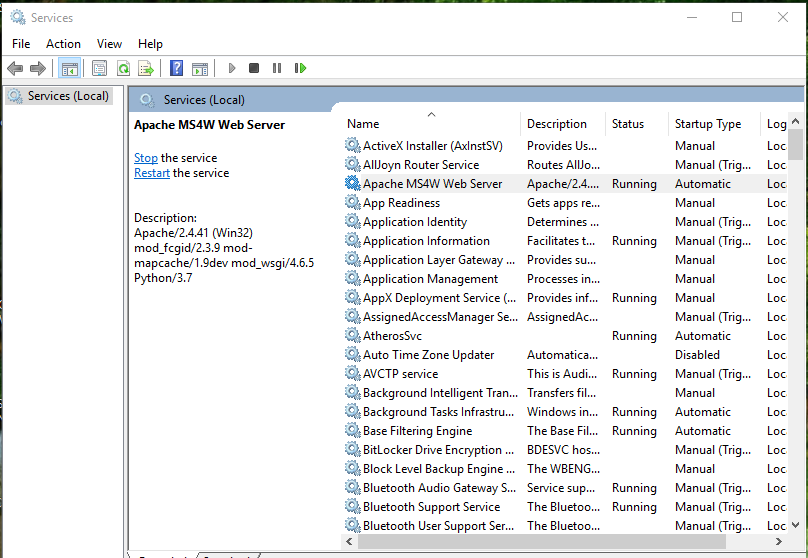
\includegraphics[width=4cm]{figures/1174015/4/No5.png}
		\centering
		\caption{Isi Folder Conf}
    \end{figure}

  \item Buka file httpd.conf dan ubah listen port nya. Karena dikomputer saya port 80 digunakan untuk webserver, port ini juga bisa d setting saat proses instalasi sebelumnya.
  \hfill\break
    \begin{figure}[H]
		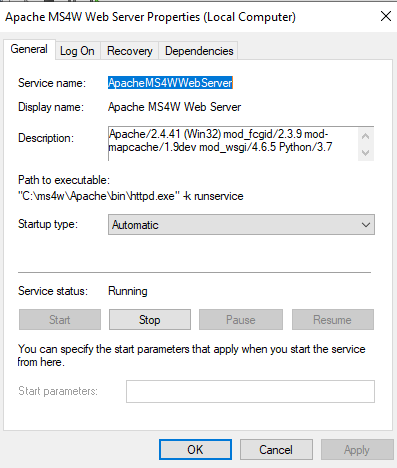
\includegraphics[width=4cm]{figures/1174015/4/No6.png}
		\centering
		\caption{Listen port}
    \end{figure}

  \item Kemudian kita jalankan servisnya, dengan menggunakan tombol windows + r dan ketikan services.msc
  \hfill\break
    \begin{figure}[H]
		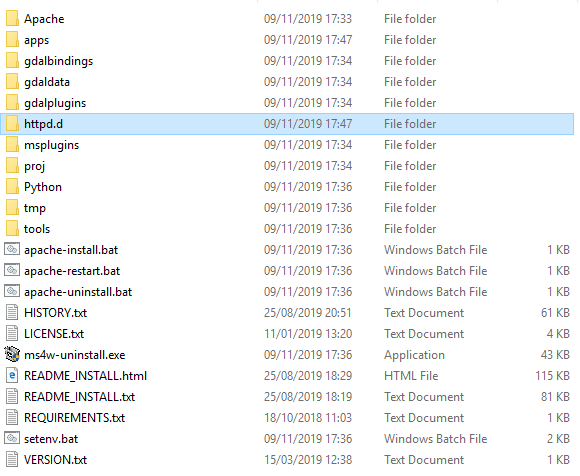
\includegraphics[width=4cm]{figures/1174015/4/No7.png}
		\centering
		\caption{Mengakses Halaman Service}
    \end{figure}

  \item Cari servis untuk Apache MS4W Web Server
    \begin{figure}[H]
		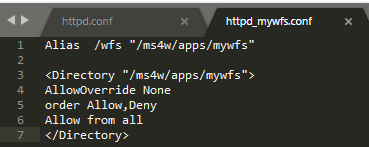
\includegraphics[width=4cm]{figures/1174015/4/No8.png}
		\centering
		\caption{Pengaturan Service Apache MS4W Web Server}
    \end{figure}

  \item Jika sudah menemukannya klik 2x
  \item Dan setting seperti berikut
  \hfill\break
    \begin{figure}[H]
		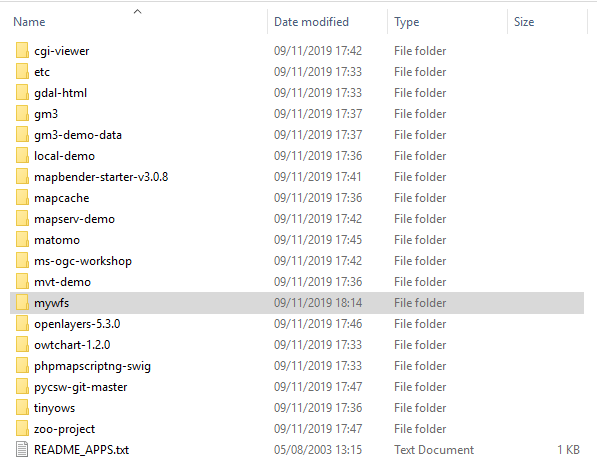
\includegraphics[width=4cm]{figures/1174015/4/No9.png}
		\centering
		\caption{Pengaturan Service Apache MS4W Web Server}
    \end{figure}

\end{enumerate}


\subsection{Pengujian}
\begin{enumerate}
  \item Masuk Ke folder httpd.d yang ada di folder ms4w
  \hfill\break
    \begin{figure}[H]
		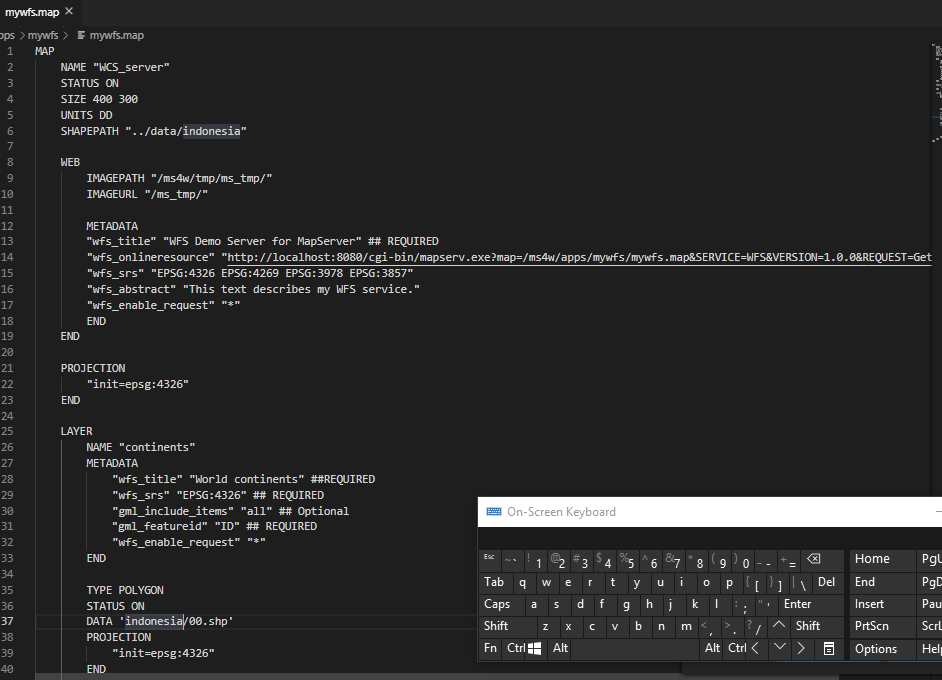
\includegraphics[width=4cm]{figures/1174015/4/No10.png}
		\centering
		\caption{Folder httpd.d}
    \end{figure}

  \item Buat sebuah file dengan nama httpd mywfs conf
  \hfill\break
    \begin{figure}[H]
		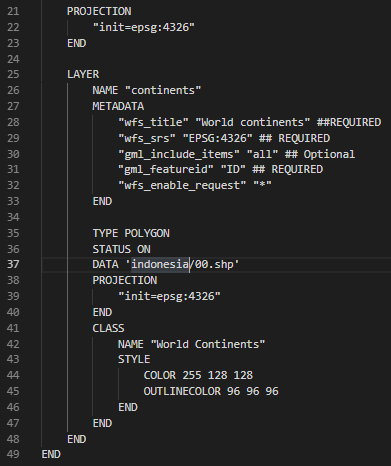
\includegraphics[width=4cm]{figures/1174015/4/No11.png}
		\centering
		\caption{Membuat file baru}
    \end{figure}

  \item Buat sebuah folder baru disana dengan nama mywfs,karena sebelumnya menyeting di httpd mywfs conf nya seperti itu
  \hfill\break
    \begin{figure}[H]
		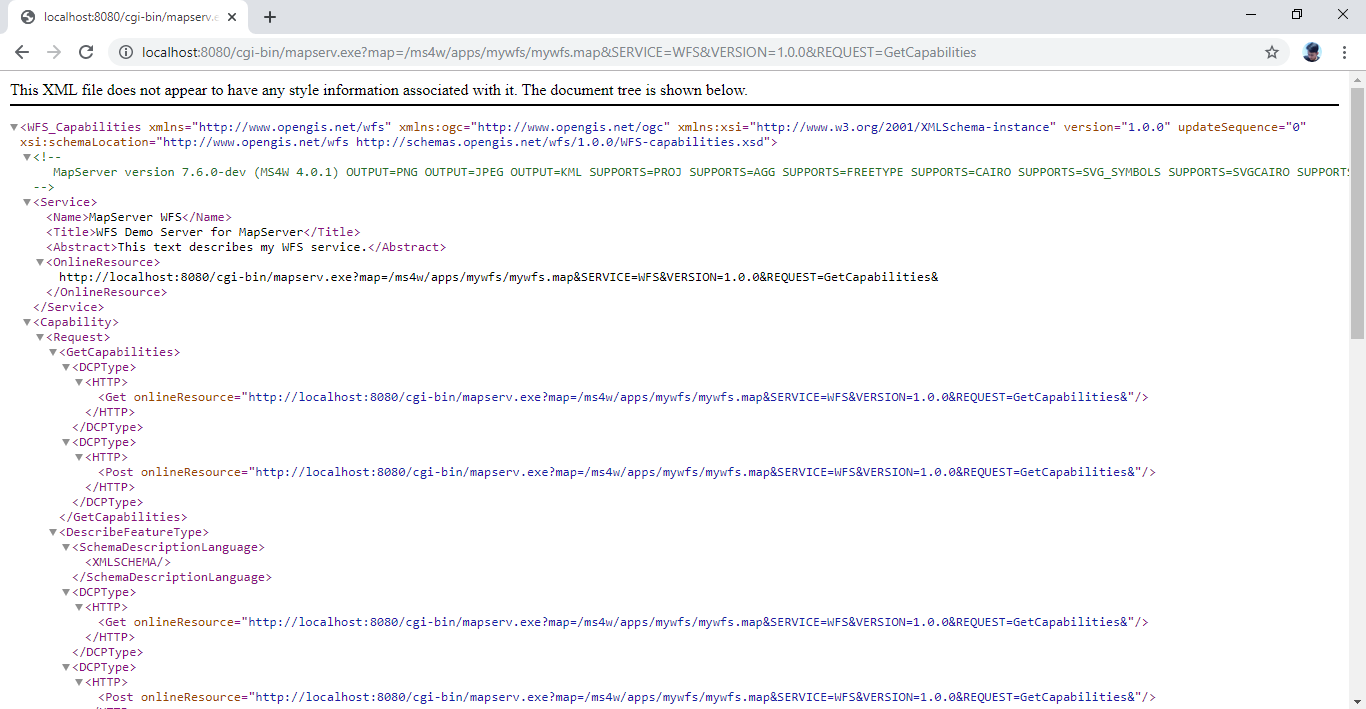
\includegraphics[width=4cm]{figures/1174015/4/No12.png}
		\centering
		\caption{Membuat folder baru}
    \end{figure}

  \item Di dalam folder mywfs buat file baru dengan nama mywfs.map
  \hfill\break
    \begin{figure}[H]
		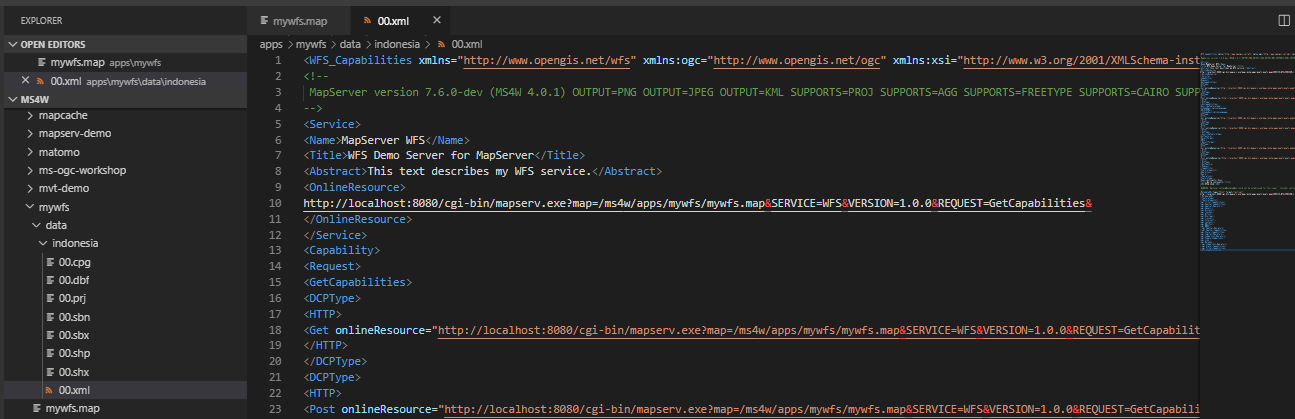
\includegraphics[width=4cm]{figures/1174015/4/No13.png}
		\centering
		\caption{Isi mywfs.map 1}
    \end{figure}

  \item Modifikasi isinya menjadi sebagai berikut
  \hfill\break
    \begin{figure}[H]
		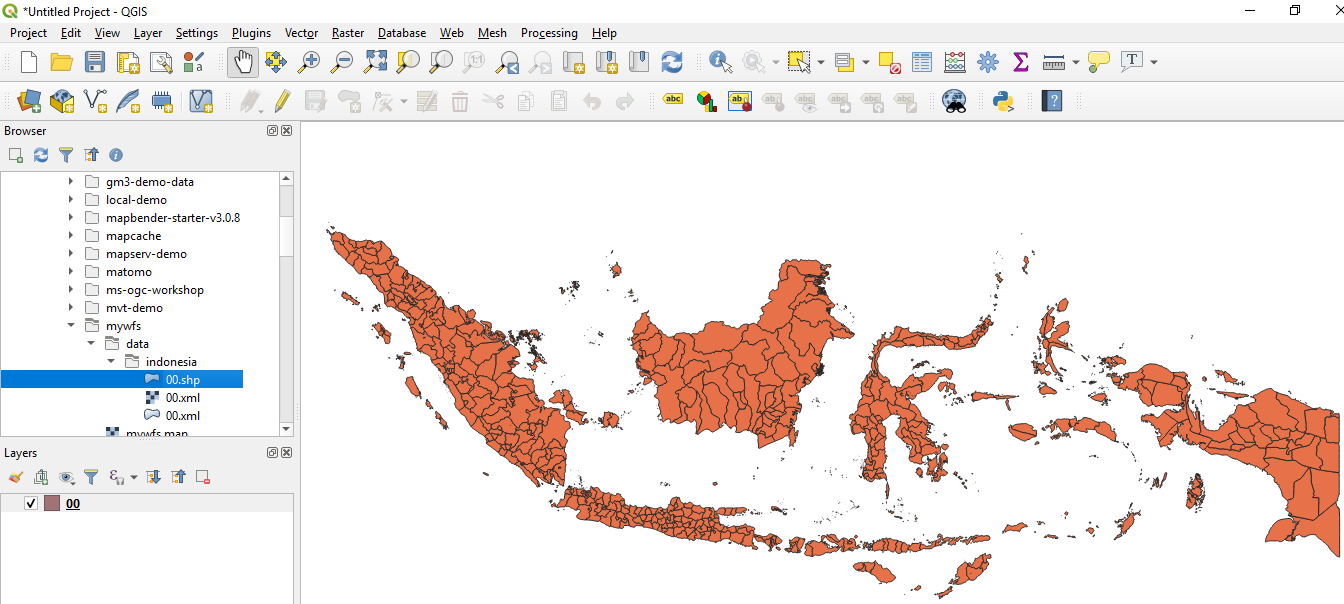
\includegraphics[width=4cm]{figures/1174015/4/No14.png}
		\centering
		\caption{Isi mywfs.map 1}
    \end{figure}

 
\end{enumerate}
\subsection{Link Youtube}
\href{https://youtu.be/TnPKz8Z2bj4}{Klik disini}